\documentclass[a4paper]{article}
\usepackage[utf8]{inputenc}
\usepackage{listings}
\usepackage{xcolor}

\lstdefinestyle{jsonStyle}{
    backgroundcolor=\color{white},
    basicstyle=\ttfamily\small,
    breaklines=true,
    captionpos=b,
    commentstyle=\color{gray},
    keywordstyle=\color{blue},
    stringstyle=\color{red},
    frame=single,
    numbersep=5pt,
    numberstyle=\tiny\color{gray},
    showspaces=false,
    showstringspaces=false,
    showtabs=false,
    tabsize=2,
    language=
}

\usepackage[margin=20mm]{geometry}
\usepackage{titlesec}
\usepackage{xcolor}
\usepackage{longtable}
\usepackage{graphicx}
\usepackage{advdate}
\usepackage{cmbright}
\usepackage{array}
\usepackage{makecell}


\definecolor{UnipdRed}{RGB}{155, 0, 20}

\usepackage{sectsty}
%\setcounter{secnumdepth}{0}
\allsectionsfont{\sffamily\color{UnipdRed}}


\usepackage{fancyhdr}
\pagestyle{fancy}
\renewcommand{\headrulewidth}{0pt}
\renewcommand{\footrulewidth}{0pt}
\setlength\headheight{80.0pt}
\addtolength{\textheight}{-80.0pt}
\chead{
\includegraphics[width=0.5\columnwidth]{logos/logo-unipd800.pdf}\hspace{0.25\columnwidth} 
\includegraphics[width=0.2\columnwidth]{logos/DEI.pdf}}
\cfoot{}

%\renewcommand{\maketitle}{
%\maketitle
%\thispagestyle{fancy}

%\pagebreak
%\pagestyle{plain}
%\setlength\headheight{20.0pt}
%\addtolength{\textheight}{-20.0pt}
%}

\makeatletter         
\renewcommand\maketitle{
{\raggedright 
\begin{center}

{   
    \Large\bfseries\sffamily 
    \@title}\\[4ex] 
    \Large
    \textbf{Master Degree in Computer Engineering\\
    Master Degree in ICT for Internet and Multimedia\\}
    \large
    \vspace{\baselineskip}
    \deadline{29 April}
    \vspace{30mm}
    \centering
\begin{longtable}{|p{.3\columnwidth}|p{.3\columnwidth} |p{.3\columnwidth}|} 
\hline
 \makecell{\textbf{Group Acronym}} & \multicolumn{2}{c|}{\makecell{Car Rental System }} \\ \hline
 \makecell{\textbf{Last Name}} & \makecell{\textbf{First Name}} & \makecell{\textbf{Badge Number}} \\
 \hline
 \makecell{Chemello}& \makecell{Francesco}& \makecell{2121346}\\\hline
 \makecell{Dolati}& \makecell{Elnaz}& \makecell{2071516}\\\hline
 \makecell{De Souza Farias}& \makecell{Gabriella Ingridy}& \makecell{2099980}\\\hline
 \makecell{Pellegrini}& \makecell{Luca}& \makecell{2122860}\\\hline
 \makecell{Safavi}& \makecell{Seyedreza}& \makecell{2071558}\\\hline
 \makecell{Sadin}& \makecell{Ahmad}& \makecell{2071555}\\\hline
\end{longtable}
    \end{center}}
    \thispagestyle{fancy}
    %\thispagestyle{empty}
    \pagebreak
    \pagestyle{plain}
    \setlength\headheight{25.0pt}
    \addtolength{\textheight}{-25.0pt}
}
\makeatother


\newcommand{\hw}{Homework 1 – Server-side Car Rental System}


\title{
Web Applications A.Y. \AdvanceDate[-365]\the\year{}-\AdvanceDate[365]\the\year{}\\
\vspace*{0.5\baselineskip}
\hw}

\newcommand{\deadline}[1]{Deadline: #1, \the\year{}}





\begin{document}
\maketitle

\section{Objectives}
The primary objective of our Car Rental web application project is to design and implement a robust and efficient platform aimed at facilitating the management of car rental operations. This endeavor is driven by the overarching goal of providing a comprehensive toolset to streamline daily activities for car rental companies while concurrently enhancing customer experiences within the realm of car rentals.\\
\\
Specifically, our project aims to achieve the following objectives:\\
\\
\textbf{1. Efficient Car Management:} Develop a centralized system for tracking and managing a fleet of rental cars, ensuring optimal utilization and maintenance. This objective encompasses tasks such as adding, editing, and removing vehicle listings, updating vehicle information (e.g., availability, pricing, specifications), and implementing alert mechanisms for low stock levels.\\

\textbf{2. Enhanced Customer Management:} Create a comprehensive platform for managing customer information, reservations, and communication channels. This entails facilitating seamless reservation processes for customers, enabling them to make and modify bookings effortlessly, and providing avenues for direct communication between staff and customers to address inquiries and resolve issues promptly.\\

\textbf{3. Streamlined Reservation Handling:} Implement an efficient reservation handling system that allows customers to make and modify reservations seamlessly. Staff members should be equipped with tools to review and manage reservations, ensuring efficient allocation of vehicles based on availability and customer preferences.\\

\textbf{4. Automated Billing and Invoicing: }Develop automated billing processes to generate invoices for reservations and additional services. This includes tracking payments, managing late fees, and generating financial reports for analysis and reconciliation.\\

\textbf{5. Effective Inventory Management:} Establish a centralized system for monitoring vehicle availability and generating alerts for low stock levels. The objective is to ensure that the right cars are available at the right time and location to meet customer demand, thereby optimizing inventory control and maximizing revenue potential.\\

\textbf{6. Comprehensive Reporting and Analytics:} Provide comprehensive reports and analytics on various aspects of the rental business, including reservation trends, revenue generation, and customer demographics. These insights will empower data-driven decision-making, enabling the company to refine strategies and drive business growth effectively.\\

\textbf{7. Security and Access Control: }Implement robust security measures, including role-based access control mechanisms, to safeguard sensitive functionalities and data. Ensuring authorized personnel have access to specific features will enhance overall system security and protect against unauthorized access or misuse.\\
\\
By accomplishing these objectives, our Car Rental web application endeavors to significantly enhance operational efficiency, elevate customer satisfaction levels, and position the company for long-term success and competitiveness in the dynamic car rental industry landscape.\newpage

\section{Main Functionalities}
The Car Rental web application boasts a comprehensive suite of functionalities meticulously designed to optimize rental operations and elevate customer experiences. These functionalities are structured into distinct modules, each serving a pivotal role in facilitating seamless interactions between users and the system. Our academic discourse on the main functionalities of the Car Rental web application is as follows:\\\\

\textbf{1. User Management Module}:\\
This module encompasses functionalities related to user account creation and administration. It facilitates the registration of staff members within the system, granting them unique login credentials for secure access. Administrative privileges empower designated personnel to oversee user accounts, ensuring proper access control and data security.\\

\textbf{2. Vehicle Management Module:\\}
The Vehicle Management module facilitates efficient oversight of the rental fleet. Staff members can seamlessly add, update, or remove vehicle listings, thereby maintaining accurate and up-to-date information regarding vehicle availability, pricing, and specifications. This module ensures that customers are presented with a comprehensive selection of vehicles to meet their rental needs.

\textbf{3. Reservation Handling Module:\\}
The Reservation Handling module streamlines the reservation process, enabling customers to make and modify bookings with ease. Staff members are equipped with tools to review and manage reservations, facilitating efficient allocation of vehicles based on availability and customer preferences. This module plays a pivotal role in ensuring a seamless booking experience for customers.\\

\textbf{4. Billing and Invoicing Module:\\}
 Automated billing processes are central to the Billing and Invoicing module, generating invoices for reservations and additional services. Staff members can track payments, manage late fees, and generate financial reports for analysis and reconciliation. This module enhances financial transparency and efficiency, ensuring smooth financial operations within the rental business.\\

\textbf{5. Inventory Management Module:\\}
The Inventory Management module monitors vehicle availability in real-time, generating alerts for low stock levels to facilitate timely replenishment of the fleet. By optimizing inventory control, this module ensures that the right vehicles are available at the right time and location to meet customer demand, thereby maximizing revenue potential.\\

\textbf{6. Reporting and Analytics Module:\\}
   - The Reporting and Analytics module provides comprehensive reports and analytics on various aspects of the rental business, including reservation trends, revenue generation, and customer demographics. These insights empower data-driven decision-making, enabling the company to refine strategies and drive business growth effectively.\\

\textbf{7. Security and Access Control Module:\\}
Robust security measures, including role-based access control mechanisms, are integrated into the Security and Access Control module to safeguard sensitive functionalities and data. This module ensures that only authorized personnel have access to specific features, enhancing overall system security and protecting against unauthorized access or misuse.\\\\

By incorporating these functionalities, the Car Rental web application aims to optimize rental operations, enhance customer satisfaction, and foster long-term success in the competitive car rental industry landscape.\newpage


\section{Data Logic Layer}

\subsection{Entity-Relationship Schema}
\begin{center}

\includegraphics[width=11cm, height=10cm]{ERSchema.png}

\end{center}
\begin{table}[htbp]
    \centering
    \begin{tabular}{|c|c|p{4cm}|}
    \hline
    \textbf{Entity} & \textbf{Attributes} & \textbf{Description} \\
    \hline
    Customer & Customer\_ID & Identifier for the customer \\
             & First Name & First name of the customer \\
             & Last Name & Last name of the customer \\
             & Email & Email address of the customer \\
             & Date of Birth & Birth date of the customer \\
             & Phone & Phone number of the customer \\
             & Password & Password for customer login \\
             & Nationality & Nationality of the customer \\
             & Address & Address of the customer \\
    \hline
    License & License\_number & Identifier for the license \\
            & Issuing\_date & Date of issuing the license \\
    \hline
    Car & Car\_ID & Identifier for the car \\
        & BrandName & Brand name of the car \\
        & ModelName & Model name of the car \\
        & Capacity & Capacity of the car \\
        & CurrentStatus & Current status of the car \\
        & Category & Category of the car \\
    \hline
    Rental Transaction & Payment\_ID & Identifier for the payment \\
                       & From\_date & Start date of rental \\
                       & To\_date & End date of rental \\
                       & Amount & Rental amount \\
                       & Payment\_status & Status of payment \\
    \hline
    Admin & Admin\_ID & Identifier for the admin \\
          & Type\_accept & Acceptance type \\
          & B1 & B1 code \\
          & Expiration\_date & Expiration date of license \\
          & E-mail & Email address of the admin \\
    \hline
    \end{tabular}
    \caption{Entity-Attribute-Description Table for ER Schema}
    \label{tab:er-schema}
\end{table}





\subsection{Other Information}

%if needed write here other details about your Data Logic Layer that cannot be expressed directly through the ER schema

The Entity-Relationship (ER) schema for the Car Rental web application outlines key entities, their attributes, and relationships:\\

\textbf{Entities:} Customer, License, Car, Rental Transaction, Admin.\\
\textbf{Relationships:} HoldsLicense, Reserve, Manage.\\
\textbf{Attributes:} Unique identifiers (IDs), customer details, rental information, administrative data.
Normalization: Ensures data integrity and efficiency.\\\\

This schema serves as the foundation for organizing and managing data within the application, supporting seamless rental operations and administrative functions.

\newpage
\section{Presentation Logic Layer}

%What pages will be present in your project? briefly indicate how your web site will be organized
In our Car Rental web application's Presentation Logic Layer, we've crafted intuitive pages to streamline user interaction:\\

\begin{itemize}
    \item The Registration Page allows swift account creation.
    \item The Add Cars Page simplifies fleet management.
    \item The User Dashboard offers personalized account insights.
    \item My Rental Cars Page facilitates document uploads.
    \item The Car Information Page provides detailed rental insights.
    \item The Home Page serves as a user-friendly entry point.\\
\end{itemize}

This setup ensures a seamless user experience and efficient navigation throughout the platform.

\subsection{Home Page}

%For the main pages put a mockup and describe it in detail.

\begin{figure}[h]
\centering
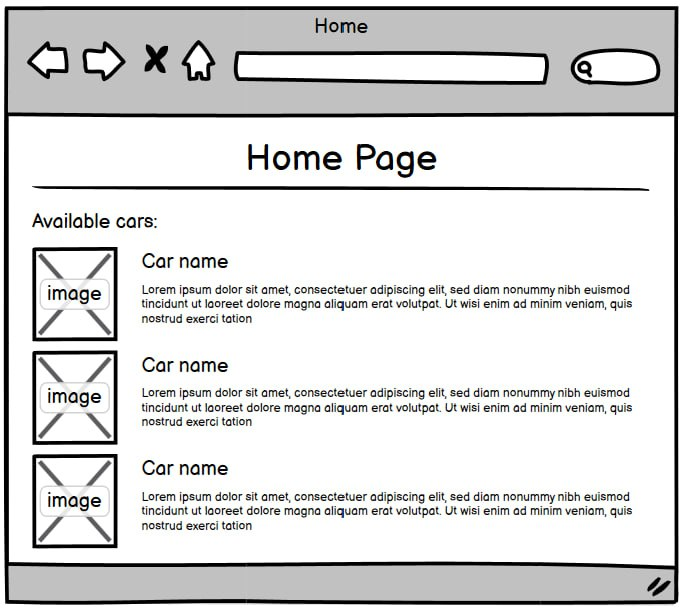
\includegraphics[width=0.7\textwidth, inner]{sections/HomePage.jpg}
\caption{Home Page}
\end{figure}\\
The Home Page serves as the main entry point, welcoming users with an overview of available cars, promotions, and featured vehicles. It provides a search and browsing interface, user sign-in options, customer testimonials, and informational resources to guide users seamlessly through the platform.\newpage
 \subsection{Registration Page: }

%For the main pages put a mockup and describe it in detail.

\begin{figure}[h]
\centering
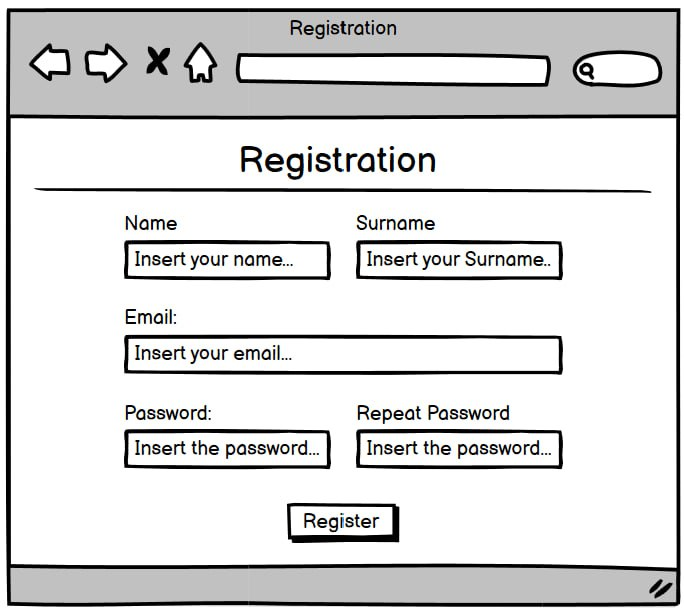
\includegraphics[width=0.7\textwidth, inner]{sections/Registration.jpg}
\caption{Registration Page}
\end{figure}\\

The Registration Page allows new users to create accounts by providing essential information such as their name, email address, password, and contact details. The registration form is user-friendly and intuitive, guiding users through the process step by step. Once the form is submitted, the user's account is created, and they gain access to personalized features and functionalities within the application. The Registration Page may also include optional fields for users to provide additional information, such as their preferences or interests, to tailor their experience further. Robust validation ensures that all entered data is accurate and secure, protecting user privacy and preventing fraudulent.\newpage
 \subsection{Add Cars Page: }

%For the main pages put a mockup and describe it in detail.

\begin{figure}[h]
\centering
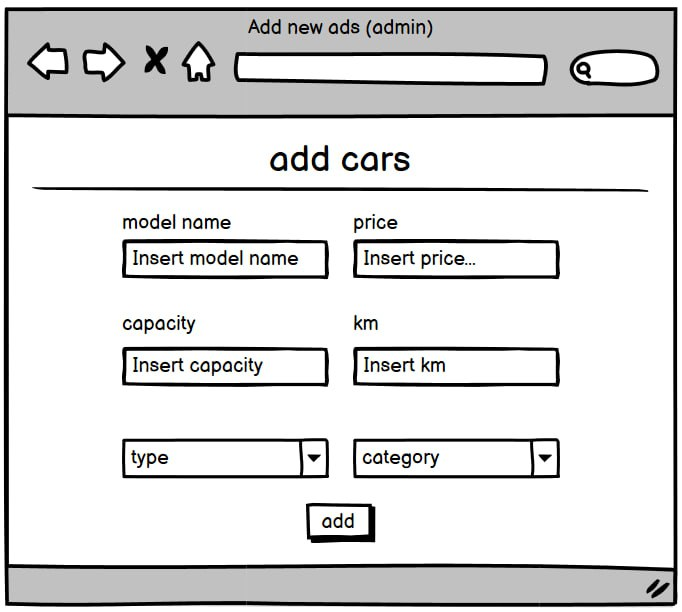
\includegraphics[width=0.7\textwidth, inner]{sections/AddCars.jpg}
\caption{Add Cars Page}
\end{figure}\\

The Add Cars Page is accessible to administrators or authorized users responsible for managing the rental fleet. It features a comprehensive form where users can input detailed information about new cars to be added to the inventory. The form includes fields for the car's license plate number, rental rate, capacity, model name, category, current status, brand name, and any additional specifications or features. Users can upload photos of the car to provide visual representations for potential renters. Once the form is submitted, the new car is added to the rental inventory, and its details are updated in the database. The Add Cars Page streamlines the process of adding new vehicles, ensuring that the rental fleet remains up-to-date and well-maintained.\newpage
 \subsection{User Dashboard:  }

%For the main pages put a mockup and describe it in detail.

\begin{figure}[h]
\centering
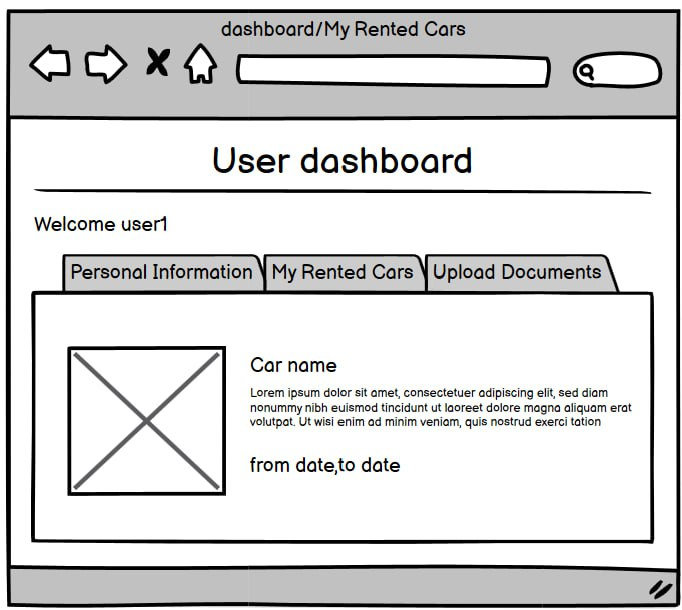
\includegraphics[width=0.7\textwidth, inner]{sections/UserDashboard.jpg}
\caption{User Dashboard Page}
\end{figure}\\


The User Dashboard serves as a centralized hub where registered users can access and manage their account information. It provides a personalized view of the user's profile, including their name, contact details, rental history, and preferences. Users can easily update their profile information, such as changing their password or updating their contact information, directly from the dashboard. The dashboard also displays any ongoing rental transactions, including the dates, duration, and status of each rental. Users can track their rental history, view past transactions, and access digital copies of rental agreements or receipts. The User Dashboard enhances user engagement and satisfaction by providing a convenient and intuitive interface for managing account activities and rental-related tasks.\newpage
 \subsection{Car Information Page:  }

%For the main pages put a mockup and describe it in detail.

\begin{figure}[h]
\centering
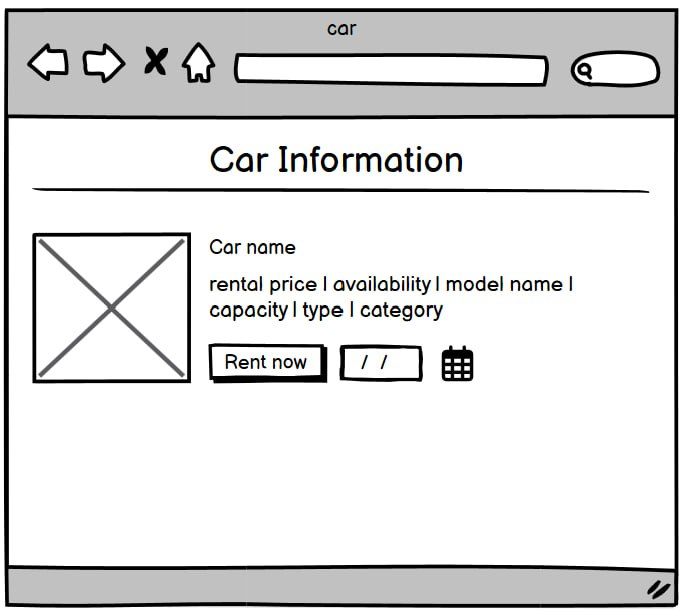
\includegraphics[width=0.7\textwidth, inner]{sections/CarInformation.jpg}
\caption{Car Information Page}
\end{figure}\\
The Car Information Page provides detailed insights into individual cars available for rental. It features comprehensive information about each car, including specifications, features, rental history, and associated fees. Users can view high-quality photos of the car from different angles to get a better understanding of its appearance and condition. The page includes detailed descriptions of the car's make, model, year, mileage, and any special features or amenities it may have. Users can also see the availability of the car for their desired rental dates and check the rental rates and fees associated with renting the car. Clear call-to-action buttons prompt users to initiate the rental process, such as requesting a reservation or contacting customer support for assistance. The Car Information Page helps users make informed decisions about their rental choices by providing comprehensive and detailed information about each car in the rental inventory.\newpage

 
 
 
 
 


\newpage
\section{Business Logic Layer}
\subsection{Class Diagram}

\includegraphics[width=500, height=350]{wa2324-homework-template/FinalClassDiagam.png}

%Describe here the class diagram of your project
\begin{table}[htbp]
    \centering
    \begin{tabular}{|p{3cm}|p{10cm}|}
    \hline
    \textbf{Component} & \textbf{Description} \\
    \hline
    DAO & Data Access Objects (e.g., `AddRentalTransactionDAO`, `AdminLoginDAO`) facilitate interactions with data storage, enabling seamless data retrieval and manipulation for rental transactions, user authentication, and vehicle listings. \\
    REST & RESTful resources (e.g., `AbstractRR`, `CreateCarRR`) serve as API endpoints, defining and handling incoming requests to provide functionalities such as creating cars and listing available vehicles. \\
    Service Layer & Classes (e.g., `Admin`, `Car`, `RentalTransaction`) encapsulate business logic for administrative tasks, vehicle management, and rental transactions, facilitating efficient operation of the application. \\
    Servlets & Servlets (e.g., `AdminLoginServlet`, `CreateCarServlet`) handle HTTP requests and responses, serving as entry points for processing user interactions and orchestrating communication between the client and server. \\
    \hline
    \end{tabular}
    \caption{Class Diagram Components}
    \label{tab:class-diagram}
\end{table}


\subsection{Sequence Diagram}
\\\\
\begin{figure}[h]
\centering
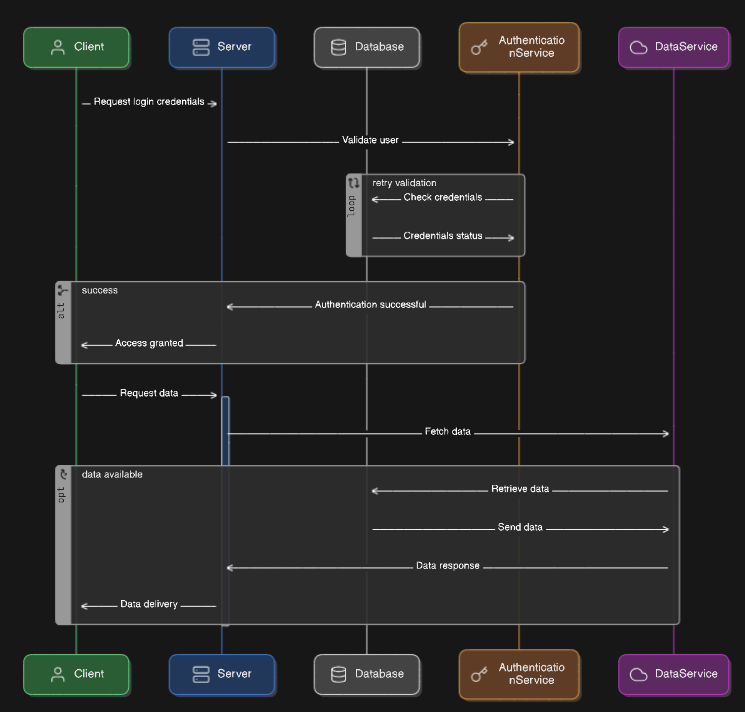
\includegraphics[width=0.8\textwidth, inner]{sections/BLL/LoginSequenceDiagram.png}
\caption{Login Sequence diagram}
\end{figure}\\
\textbf{Description:}\\ The login process begins when the client sends a request to the server with the user's credentials. The server verifies the provided username and password against stored data. If the credentials are valid, the server responds with a success message, granting the user access. This sequence diagram outlines the essential steps involved in the login process and emphasizes the importance of authentication for system security.\newpage

\begin{figure}[h]
\centering
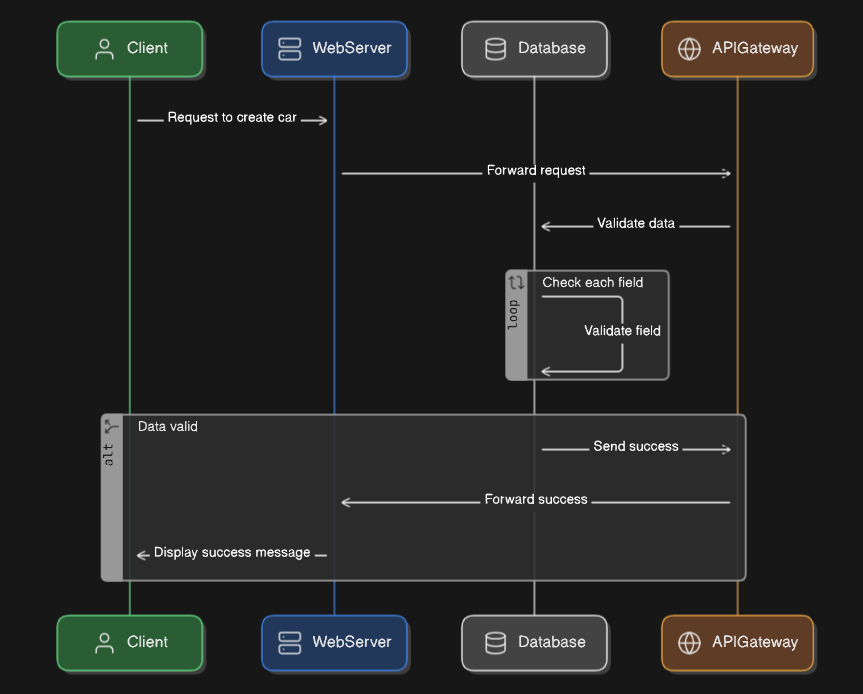
\includegraphics[width=0.8\textwidth, inner]{sections/BLL/CarSequenceDiagram.png}
\caption{Car Sequence Diagram}
\label{fig:figure2}
\end{figure}
\textbf{Description:}\\
The car sequence diagram illustrates the process flow involved in managing cars within the system. It visually depicts the interactions between various components, including clients, servlets, DAOs (Data Access Objects), resources, and databases.\\
In this sequence, the client initiates the process by sending a request to the server, often facilitated by a servlet. The servlet then communicates with the appropriate DAO to perform operations related to cars, such as creation, updating, or reservation. The DAO interacts with the database to retrieve or modify car-related data accordingly.\\
For instance, in a car reservation scenario, the sequence might show the client requesting to reserve a car. The servlet processes this request and communicates with the reservation DAO to verify car availability and update the reservation status in the database. Finally, the servlet responds to the client, indicating the success or failure of the reservation process.\\
Overall, the car sequence diagram provides a visual representation of the steps involved in managing cars within the system, aiding in understanding the process flow and interactions between different system components.\newpage
\begin{figure}[h]
\centering
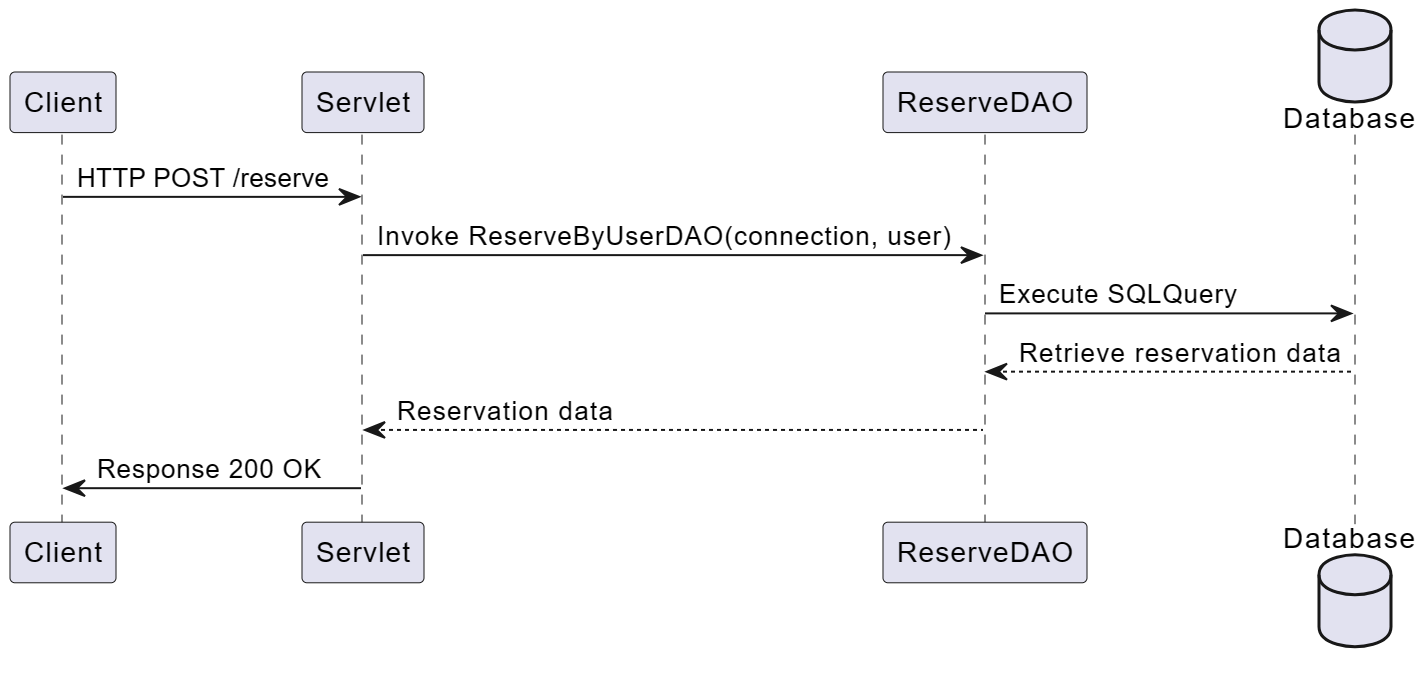
\includegraphics[width=0.9\textwidth, inner]{sections//BLL/Reserve-Sequence-diagram.png}
\caption{Reserve Sequence Diagram}
\label{fig:figure2}
\end{figure}
%describe here the sequence diagram
\textbf{Description:}\\
The car reservation sequence diagram illustrates the process of reserving a car within the system.\\
The client initiates the process by sending an HTTP POST request to the servlet, triggering a series of interactions. The servlet interacts with the ReserveDAO to access the database and retrieve reservation data for the specified user. Following this, the database processes the request, retrieves the necessary data, and returns it to the servlet. Finally, the servlet responds to the client with an HTTP status code of 200 OK, indicating a successful reservation.\\
This sequence diagram provides a clear overview of the interactions involved in the car reservation process, from client request to server response.\newpage
\subsection{REST API Summary}

%describe the REST API. If needed, add a few lines of text here, describing the content of the table.
We used postman REST client to test and debug our REST API. here we share list of routes and a documentation with other developers: 

\begin{longtable}{|p{.225\columnwidth}|p{.1\columnwidth} |p{.30\columnwidth}|p{.30\columnwidth}|} 
\hline
\textbf{URI} & \textbf{Method} & \textbf{Description} & \textbf{Filter} \\\hline

/rest/car & GET &  get the list of cars & no \\\hline

/rest/car & POST &  make a new car record & no \\\hline

/rest/car/\{licenseplate\} & GET &  get a car by its license plate & filters cars by license plate \\\hline

/create-car & POST &  make a new car record & no \\\hline

/update-car & POST &  update a car record & no \\\hline

/search-car & GET &  get the list of cars & can filter with cars parameters \\\hline

/create-customer & POST &  Registering a new customer & no \\\hline

/edit-customer & POST &  Registering a new customer & no \\\hline

/login & POST &  Login a customer & no \\\hline

/create-licence & POST &  Creating a new Licence & no \\\hline

/edit-licence & POST &  update a car record & no \\\hline

/add-transaction & POST &  create a payment transaction & no \\\hline

/remove-transaction & POST &  remove a payment transaction & no \\\hline

/update-transaction & POST &  remove a payment transaction & no \\\hline


\caption{Describe in this table your REST API}
\label{tab:termGlossary}
\end{longtable}
\subsection{REST Error Codes}

%If needed, add few lines of text, describing the error codes table

\begin{longtable}{|p{.35\columnwidth}|p{.2\columnwidth} |p{.4\columnwidth}|} 
\hline
\textbf{Error Code} & \textbf{HTTP Status Code} & \textbf{Description} \\\hline

E300 - E4A1 - E4A3 - E4A7 & 400 &  Bad Request\\\hline
E404 - E5A3 & 404 &  Not Found\\\hline
E4A5 & 405 & Method Not Allowed \\\hline 
E4A2 & 406 & Not Acceptable \\\hline 
E5A2 - E5A4 & 409 &  Conflict\\\hline
E4A4 & 415 &  Unsupported Media Type \\\hline
E200 - E5A1 & 500 &  Internal Server Error\\\hline

\caption{Describe in this table your REST API}
\label{tab:termGlossary}
\end{longtable}\newpage
\subsection{REST API Details}

%List here a few resources retrievable via REST API

\subsubsection*{Register Form}

% the description of the resource

REST API details for the Register form include endpoints and request/response formats for handling user registration. The form collects essential user details such as email, first name, last name, birth date, address, phone number, nationality, password, and license number.



\begin{itemize}
    \item URL: \texttt{/createCostumer}
    \item Method: \texttt{Post}
    % \item URL Parameters:
    \item Data Parameters: \\
\begin{figure}[h]
\centering
\includegraphics[width=0.8\textwidth, inner]{sections//BLL//DataParameter1.jpg}
\caption{Register Form Data Parameter}
\label{fig:figure1}
\end{figure}
    \item Success Response:
\begin{figure}[h]
\centering
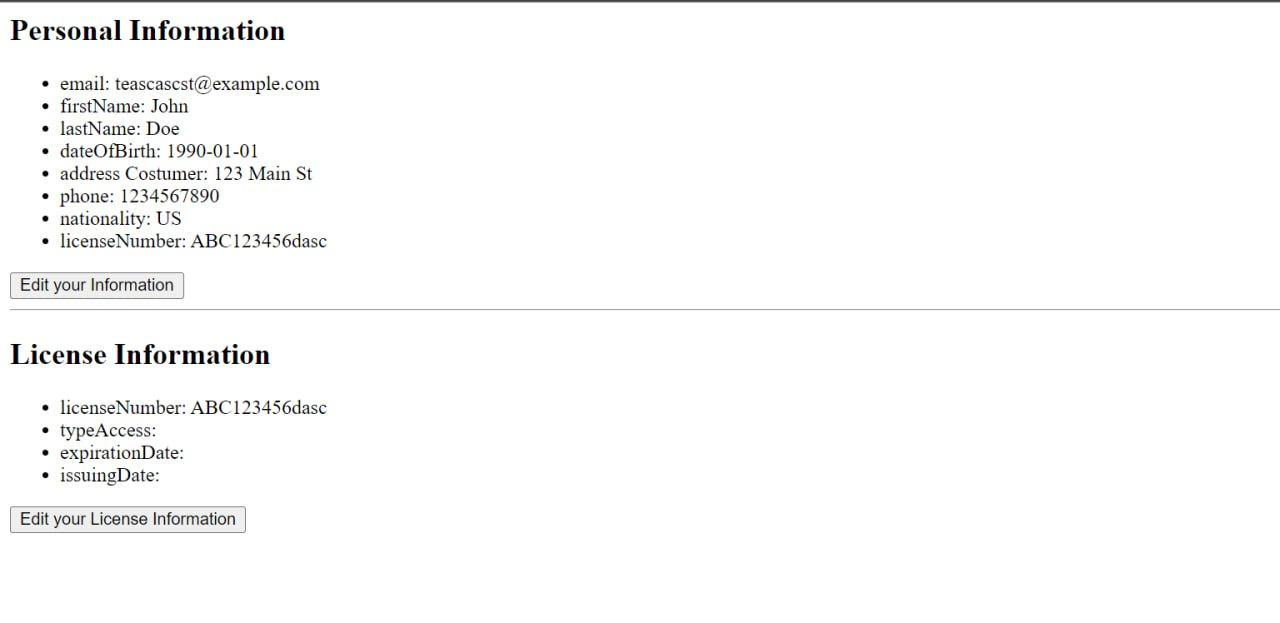
\includegraphics[width=0.8\textwidth, inner]{sections//BLL/SuccssResponse1.jpg}
\caption{Create Costumer Success Response}
\label{fig:figure2}
\end{figure}\newpage
    % \item Error Response:
\subsubsection*{Update Car}
    \item URL: \texttt{/updateCar}
    \item Method: \texttt{Post}
    % \item URL Parameters:
    \item Data Parameters: \\
\begin{figure}[h]
\centering
\includegraphics[width=0.8\textwidth, inner]{sections//BLL/DataParameter1.jpg}
\caption{update Car Data Parameter}
\label{fig:figure1}
\end{figure}
    \item Success Response:
\begin{figure}[h]
\centering
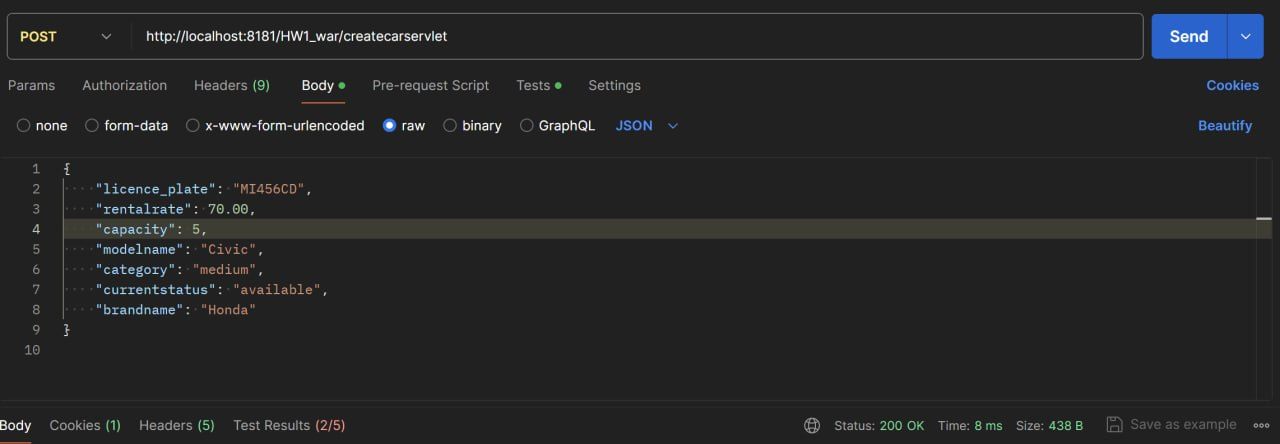
\includegraphics[width=0.7\textwidth, inner]{sections//BLL/updateCar1.jpg}
\caption{Update Car Success Response}
\label{fig:figure1}
\end{figure}\newpage
\newpage
    
\end{itemize}

\subsubsection*{CAR REST APIs}
Here we show some spesific REST API endpoints for managing the car entity. this APIs are under "/rest/car" URL:

\begin{itemize}
    \item URL: \texttt{the URL to retrieve it : /rest/car}
    \item Method: \texttt{Method to retrieve it: GET}
    \item URL Parameters: none
    \item Data Parameters: none
    \item Success Response: 
        \begin{lstlisting}[ style=jsonStyle, caption={ Response Example }, label={lst:json}]
        {
          "resource-list": [
            {
              "car": {
                "licenseplate": "HR23791B",
                "rentalrate": 50.0,
                "capacity": 5,
                "category": "medium",
                "currentstatus": "available",
                "brandname": "Toyota"
              }
            },
            {
              "car": {
                "licenseplate": "T6237FX5",
                "rentalrate": 70.0,
                "capacity": 4,
                "category": "small",
                "currentstatus": "available",
                "brandname": "Honda"
              }
            }
          ]
        }
        \end{lstlisting}
        
    \item Error Response: 
        \begin{lstlisting}[ style=jsonStyle, caption={ Possible Errors }, label={lst:json}]
        500 :  Internal Server Error
    \end{lstlisting}

    
\end{itemize}

\begin{itemize}
    \item URL: \texttt{the URL to retrieve it : /rest/car}
    \item Method: \texttt{Method to retrieve it: POST}
    \item URL Parameters: none
    \item Data Parameters: 
      \begin{lstlisting}[ style=jsonStyle, caption={ Response Example }, label={lst:json}]
        {
            "car":{
            "licenseplate":"H3361WE0",
            "rentalrate": 60.0,
            "capacity": 4,
            "category":"medium",
            "currentstatus":"available",
            "modelname": "X5",
            "brandname": "BMW"
        
            }
        }
        
        \end{lstlisting}
    \item Success Response: 
        \begin{lstlisting}[ style=jsonStyle, caption={ Response Example }, label={lst:json}]
       {
            "car":{
            "licenseplate":"H3361WE0",
            "rentalrate":60.0,
            "capacity":4,
            "category":"medium",
            "currentstatus":"available",
            "brandname":"BMW"
            }
        }
        \end{lstlisting}
    \item Error Response: 
        \begin{lstlisting}[ style=jsonStyle, caption={ Possible Errors }, label={lst:json}]
        500 :  Internal Server Error (Cannot create the car: unexpected error. | Cannot create the car: unexpected database error.)
        400 : Bad Request (Cannot create the car: no Car JSON object found in the request.)
        409: Conflict (Cannot create the car: it already exists.)
        \end{lstlisting}
\newpage
    
\end{itemize}

\begin{itemize}
    \item URL: \texttt{the URL to retrieve it : /rest/car/\{licenceplate\}}
    \item Method: \texttt{Method to retrieve it: GET}
    \item URL Parameters: none
    \item Data Parameters:none
    \item Success Response: 
        \begin{lstlisting}[ style=jsonStyle, caption={ Response Example }, label={lst:json}]
       {
            "car":{
            "licenseplate":"H3361WE0",
            "rentalrate":60.0,
            "capacity":4,
            "category":"medium",
            "currentstatus":"available",
            "brandname":"BMW"
            }
        }
        \end{lstlisting}
    \item Error Response: 
        \begin{lstlisting}[ style=jsonStyle, caption={ Possible Errors }, label={lst:json}]
        500 :  Internal Server Error (Cannot get car: unexpected error. | Cannot get car(s): unexpected database error.)
        \end{lstlisting}
\newpage
    
\end{itemize}

\newpage
    
\end{itemize}

\begin{itemize}
    \item URL: \texttt{the URL to retrieve it : /rest/car/\{licenceplate\}}
    \item Method: \texttt{Method to retrieve it: DELETE}
    \item URL Parameters: none
    \item Data Parameters:none
    \item Success Response: 
        \begin{lstlisting}[ style=jsonStyle, caption={ Response Example }, label={lst:json}]
       {
            "car":{
            "licenseplate":"H3361WE0",
            "rentalrate":60.0,
            "capacity":4,
            "category":"medium",
            "currentstatus":"available",
            "brandname":"BMW"
            }
        }
        \end{lstlisting}
    \item Error Response: 
        \begin{lstlisting}[ style=jsonStyle, caption={ Possible Errors }, label={lst:json}]
        500 :  Internal Server Error (Cannot delete the car: unexpected database error.)
        404 : Not Found ("Car " + lisenceplate + " not found. Cannot delete it." | Cannot delete the car: wrong format for URI /car/{licenceplate}.)
        409: Conflict (Cannot delete the car: other resources depend on it.)
        
        \end{lstlisting}
\newpage
    
\end{itemize}



\section{Group Members Contribution}

% For each group member, describe in detail the contribution to the project.

\begin{description}
	\item[Francesco Chemello
] played a pivotal role in our group project, contributing extensively across various domains. He led the development of essential components such as the Car DAO, Card DAO, Rental Transaction DAO, Search DAO, Expired License DAO, Expired Reservation DAO, and Undo Reservation DAO. In addition to these backend implementations, Francesco spearheaded the creation of service layers, encompassing functionalities related to Car, Card, Rental Transaction, and Reserve Services. His expertise also extended to servlet implementations, where he meticulously handled all aspects concerning Car, Card, and Rental Transaction functionalities. On the database front, Francesco contributed significantly by designing the ER schema and ensuring thorough documentation by adjusting code for JavaDoc generation. Furthermore, he undertook crucial code maintenance tasks, addressing issues in files like BasicDAO, Actions, Abstract Database Servlet, Web.xml, and Maven Configuration/POM. To guarantee seamless integration, Francesco conducted comprehensive testing using Maven to validate the code's packaging and functionality within our project framework.
	\item[Elnaz Dolati]As a crucial member of our team, I played a pivotal role in shaping the foundation and functionality of our project. I took the lead in setting up the initial project structure, ensuring it was conducive to smooth development and collaboration. Additionally, I focused on building a secure authentication system to safeguard our project's integrity. In terms of documentation, I made significant contributions to the project report, particularly in detailing the CAR REST APIs, where I provided thorough insights and explanations.
	\item[Gabriella Ingridy De Souza Farias
	] Contribution on ER schema, tables and insert SQL, some code of Reserve and the functionality SearchByUser.
	\item[Luca Pellegrini
]I developed all the REST API: CreateCar, DeleteCar, GetCar and ListCar creating and modifying the related DAO and servlets. I contributed to the integration of the database into the web application making necessary modifications to both the database structure and the web application code.
	\item[Seyedreza Safavi
] played a pivotal role in our project, ensuring robust database connectivity and functionality. He enabled database connection via a context.xml file and developed essential login and register servlets and DAOs, rigorously tested with sample data. Additionally, Reza implemented edit DAOs and servlets for user and license information updates, enhancing project flexibility. He optimized project performance by modifying key classes like User, License, LogContext, and Message. Notably, Reza streamlined data management by implementing a database function to write simultaneously to customer and license tables. He also created all necessary JSPs, facilitating data reception, database interaction, result display, and seamless navigation. Furthermore, Reza modified the web.xml file to effectively connect all servlets and JSPs. He conducted comprehensive testing of Francesco's DAOs and servlets, ensuring compatibility with a simplified database structure. Moreover, he handled exceptions effectively, enhancing the robustness of the application.
	\item[Ahmad Sadin
]was heavily involved in shaping the majority of the report's content. He took the lead in defining key functionalities, crafting the ER-schema, outlining objectives, establishing the data logic layer, and developing class and sequence diagrams. Additionally, Ahmad played a vital role in shaping the presentation logic layer, business logic layer, and specifying REST API details. Moreover, he closely collaborated with Seyed Reza on various tasks, including refining JSP files and implementing user servlets and DAOs. These combined efforts under Ahmad's guidance ensured the successful completion of the project and the achievement of its objectives.

\end{description}


\end{document}
